\usetikzlibrary{graphs,rdf}
\tikzset{
dfa/.style = { semithick, > = To [sep] },
nfa/.style = { semithick, > = To [sep] },
state/.style = { circle, draw, minimum size = 1cm },
final/.style = { double },
initial/.style = { draw = red }, % to keep things simple
transition/.style = { edge label = {$#1$} }
}
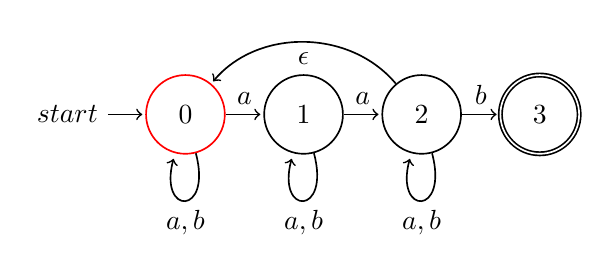
\begin{tikzpicture}[nfa]
	\graph [math nodes, grow right = 1.5cm]{
		start ->
		0 [state,initial] -> [transition = {a,b}, loop below]
		0 -> [transition=a]
		1 [state] -> [transition = {a,b}, loop below]
		1 -> [transition=a]
		2[state] -> [transition = {a,b}, loop below]
		2 -> [transition=b]
		3[state, final];
		2 -> [transition=\epsilon,out=130,in=50]
		0;
	};
\end{tikzpicture}
